\section{Bierbrau Vorgang}
\subsection{Bierarten und Brauarten}
Es gibt viele Möglichkeiten, Bier und noch mehr Biersorten zu brauen.
Bier zu brauen gibt es schon so lange, wie es Menschen gibt. Es gibt sogar Aufzeichnungen über alte Eygpten und Mesopotamien \footnote{
	Mesopotamien oder Zweistromland bezeichnet die Kulturlandschaft in Vorderasien, die durch die großen Flusssysteme des Euphrat und Tigris geprägt wird.
}.\\
Jedes Getreide, das bestimmte Zucker enthält, könnte fermentieren. Da es wilde Hefen in der Luft gibt.
Das bedeutet, dass selbst in der Zeit der Stämme, als sie mit der Landwirtschaft begannen, eine Art Bier hergestellt worden sein könnte.\\
Das meiste Bier wird aus einer Art Stärkequelle hergestellt, die fermentiert werden kann, Brauereihefe zur Herstellung und Einleitung der
Gärung und Aromatisierung wie Hopfen, um die Süße des Zuckers auszugleichen

\subsection{Bestellung}
Zur Vorbereitung des Bierbrauens benötigten wir Materialien.
Wir entschieden uns für die Verwendung von "Bier-Kits". Aus Zeitgründen war es nicht möglich,
das Bier auf traditionelle Weise zu brauen, da dies zu lange dauern würde.
Wir bestellten zwei verschiedene Kits, von denen das eine ein Cherry Ale und das andere ein belgisches Saisonbier war.
Wir haben uns für diese beiden Biere entschieden, zum einen, weil wir einen Grundtyp von Bier brauen wollten, zum anderen, weil wir etwas experimentelleres brauen wollten.  Das experimentelle ist das Cherry Ale. Wir hatten so etwas in der Schweiz noch nie so leicht erhältlich gesehen und wollten es unbedingt ausprobieren.
Der zweite Grund war die Verfügbarkeit. Wir hatten uns schon früher für Tyuoes entschieden, und sie waren nicht schnell verfügbar. Und wegen des Zeitdrucks bei diesem Projekt mussten wir das nehmen, was von Anfang an verfügbar war.

Wir hatten bereits Ausrüstung, um das Bier selbst zu brauen, wie Callum Stringer dies schon einmal getan hatte.
Unsere definitive Reihenfolge war wie folgt.

\textbf{Schon vorhandene Artikel}
\begin{itemize}
	\item Starter-Paket de Luxe für Bierkits - Preis CHF 79.00
\end{itemize}
\textbf{Neu bestellte Artikel}
\begin{itemize}
	\item Bügelflasche braun kompl. 0,5 L - Preis CHF 126.00
	\item Brewferm Bierkit Cherry Ale - Preis CHF 29.00
\end{itemize}

Als wir die Bestellung erhielten, stellten wir fest, dass uns ein Fehler unterlaufen war, und bestellten 60 Bierflaschen,
 wobei wir davon ausgingen, dass jeder Satz 15 Liter ergeben würde. Dies bedeutete, dass wir genau genug Flaschen für das gesamte Bier haben würden.
 Je nach Art des Kits war die gebraute Biermenge jedoch unterschiedlich. Wir hatten also viel zu viele Flaschen.

 \begin{figure}[!h]
	\centering
	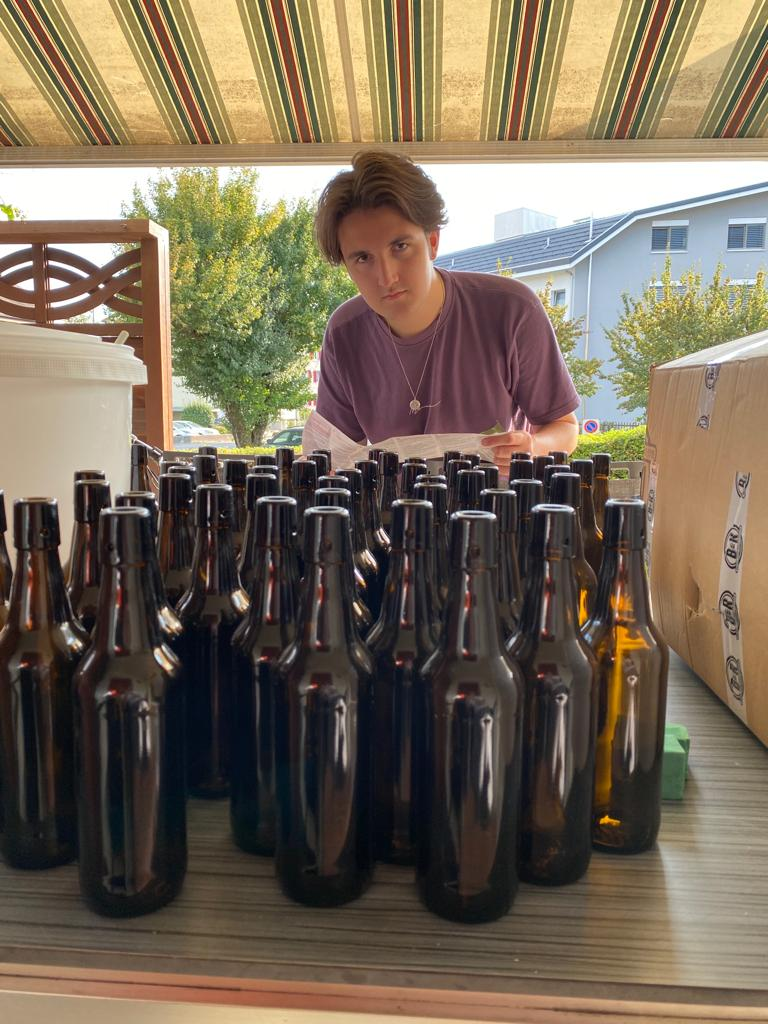
\includegraphics[width=0.5\columnwidth]{callum.png}
	\caption{Kontrolle der Bestelle Artikeln}
\end{figure}

\subsection{Vorbereiten}
\subsubsection{Disinfektion}
Zunächst einmal mussten wir alles vollständig reinigen.
Dazu bereiteten wir eine Desinfektionslösung mit den im Bierkit enthaltenen Mischgranulaten vor.
Dies war wichtig, da wir nicht wollen, dass etwas Unbekanntes im Bier ist, wenn es gärt.
Danach konnten wir mit dem eigentlichen Brauen des Bieres fortfahren. \\

Die Desinfektion hat einige Zeit in Anspruch genommen. Wir haben das Bier im Haus von Fabrizio Francos Familie gebraut.
Und Platz zu finden, um die großen Eimer durchgehend zu reinigen,
war eine echte Herausforderung. Am Ende haben wir viele der Reinigungsarbeiten in der Badewanne durchgeführt.
Hier gab es auch einige andere Herausforderungen. Die Desinfektionslösung war nicht die neutralste Flüssigkeit.
Callum Stringers dazu zu bringen, die Hände jucken und zornig zu machen. Danach entschieden wir uns für die Verwendung von Reinigungshandschuhen.
Der Prozess verlief danach sehr viel reibungsloser


\begin{figure}[!h]
	\centering
	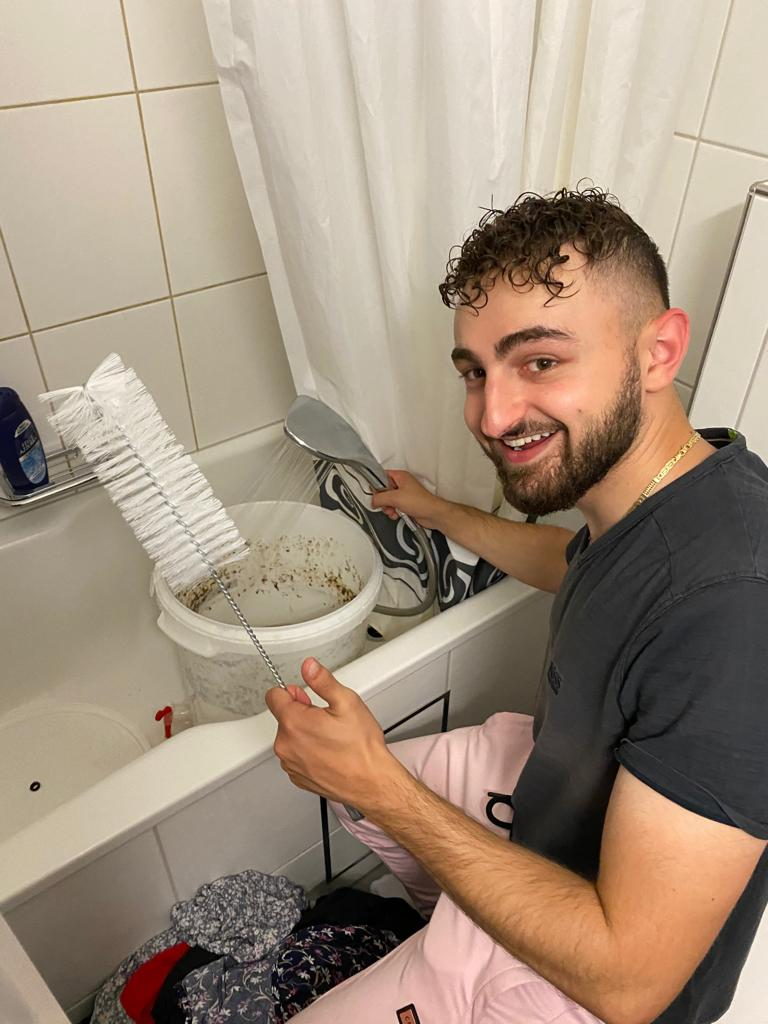
\includegraphics[width=0.5\columnwidth]{fabi.jpg}
	\caption{Disinfektion der Fass}
\end{figure}


\subsubsection{Bierkit vorbereitung}
Zuerst mussten wir die Bausätze öffnen. Nach dem Öffnen mussten wir sie aufwärmen. Dazu legten wir
sie etwa 15 Minuten lang in eine mit Wasser gefüllte Pfanne bei schwacher Hitze. Sobald es warm war,
wurde es in die großen Braubehälter gegossen. Danach fügten wir das Wasser hinzu. Je nach Art des Bierkits
geschah dies in verschiedenen Schritten. Zuerst warmes Wasser, dann lauwarmes Wasser auf die Gesamtmenge.
Einige dieser Wasserchargen waren Zuckerlösungen. Da die Hefe Zucker zum Leben und Wachsen braucht.
Danach hatten wir zwei große Fässer des jungen Bieres.
Dieses musste vor der Abfüllung gelagert werden, wir legten es in den Kasten und ließen es dort für 10 Tage stehen.
Wenn man das Bier sotriert, muss man darauf achten, wo und unter welchen Bedingungen es gelagert wird.
Damit die Hefe einwirken kann, muss die Hefe in der ersten Brauphase relitavly warm sein, jedoch nicht zu warm und ungünstig an einem dunklen Ort. 
Denn direkte Sonneneinstrahlung kann die Hefe leicht abkühlen, und ohne Hefe gibt es kein Bier!
Außerdem muss man darauf achten, dass die Flasche bzw. das Fass gut verschlossen ist. Wir haben wegen des billigen Materials,
aus dem das Fass hergestellt ist, bemerkt, dass die Möglichkeit von Undichtigkeiten besteht. Wie Sie auf dem folgenden Bild sehen können,
haben wir einige Papierzwillinge zurückgelassen, falls während der Lagerung Bier ausgelaufen sein sollte. \\



\begin{figure}[!h]
	\centering
	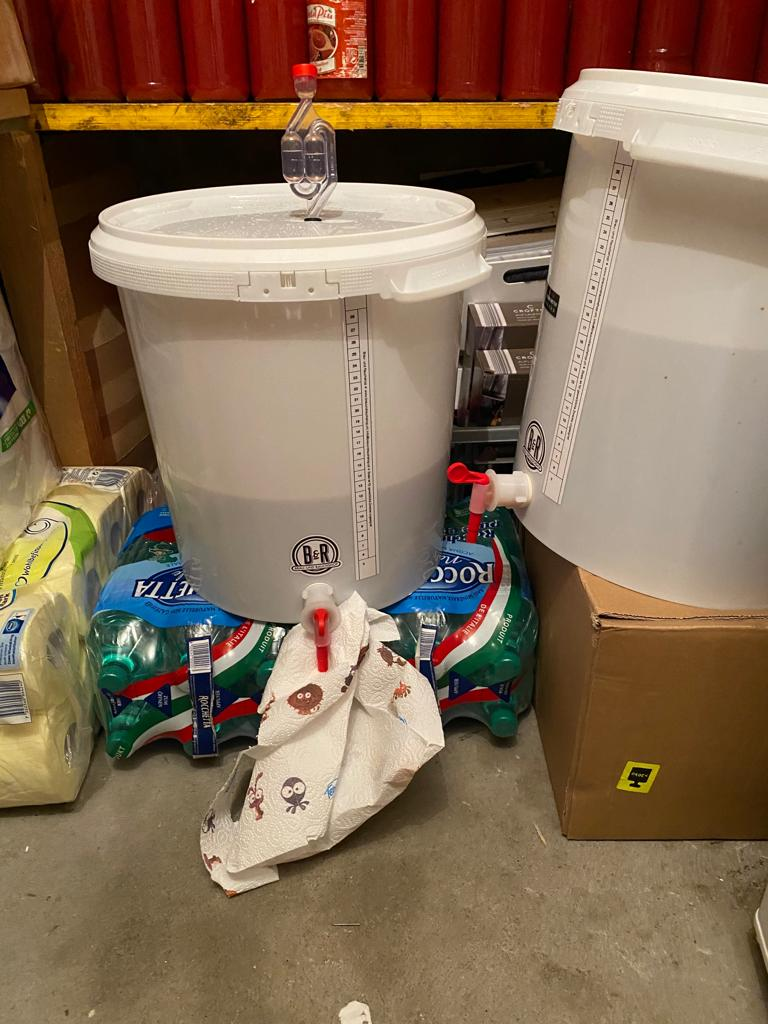
\includegraphics[width=0.5\columnwidth]{barrels.jpg}
	\caption{Lagerung der Bier}
\end{figure}
\newpage

\subsubsection{Bier in Flaschen abfüllen}
Bevor wir mit dem Abfüllen des Biers in die Glasflaschen angefangen haben, mussten wir alle neuen und alten Flaschen waschen. Wir haben 6 Liter Wasser und 5 Gram Waschmittel in einem Korb eingefüllt und gemischt. Nach 5 Minuten fingen wir an die Flaschen in dem Korb rein zu tun und liessen sie für eine Minute im Wasser stehen und spülten sie danach ab um jeden Schmutz, welcher sich in den Flaschen gesammelt hat zu entfernen. Dies dauerte länger als erwartet, da wir alle vorhandenen Flaschen gewaschen haben und diese um die 90-100 Flaschen waren. Nach dem abwaschen gaben wir jeder Flasche einen auf- und schliessbaren Deckel. Die Flaschen sahen alle gleich aus und damit wir kein durcheinander haben, fingen wir mit der Produktion von dem Cherry Ale an. Wir hatten nur 12 Liter von diesem Ale und jede Flasche hatte eine Kapazität von 0,5 Liter d.h. für 12 Liter waren es 24 Flaschen. Nachdem wir 1,5 Stunden gebraucht haben um alles zu reinigen und trocknen, haben wir die ersten 24 Flaschen auf dem Tisch gestellt. Dann fing der Spass erst an. Am Braugefäss war ein Schlauch zum Abfüllen angehängt und dieser war so präpariert, dass wenn man den Anfang des Schlauchs gegen etwas drückt fing das Bier an zu strömen und wenn kein Druck mehr stattfand hörte es auf. Durch ein Ventil welches am Braugefäss angebaut war, konnten wir den Durchfluss des Biers starten und stoppen.
Wir öffneten das Ventil, steckten den Schlauch in die Flasche und drückten es gegen den Flaschenboden bis es bis zum Flaschenhals voll mit Bier war, machten aber die Flaschen noch nicht mit dem Deckel zu weil noch eine Zutat fehlte. Nachdem wir alle 24 Cherry Ale Flaschen abgefüllt hatten verstauten wir diese für den Moment in einer Kiste und stellten die neuen Flaschen für «das andere Ale wo mir jetzt grad nid ihfallt» auf dem Tisch und führten den gleichen Vorgang erneut aus. Diese Flaschen stellten wir in eine separate Kiste. Jetzt fehlte nur noch das Einfügen des Zuckers. Dieser Vorgang war nicht so leicht und ein bisschen hektisch. Wir stellten auf den vorbereiteten Flaschen einen Trichter, zum einfüllen von einem Esslöffel Zucker. Dies musste aber eingefüllt und die Flasche schnell verschlossen werden. Wir hatten einen Zeitraum von 3 Sekunden um beides zu machen und waren wir zu langsam, schäumte das Bier über und es gab eine riesige Sauerei. Dies machten wir für alle 90 Flaschen und zum Glück geschah dies nur einmal über den ganzen Vorgang. Danach verstauten wir die Flaschen wieder getrennt in die Kisten und liessen sie für mehrere Wochen stehen.
